% =============================================================================
\section{Repaso: el x500 y PX4}
% =============================================================================

\begin{frame}{El x500 en una lámina}
  \centering
  \begin{tikzpicture}
    \node[anchor=south west,inner sep=0] (img) at (0,0) {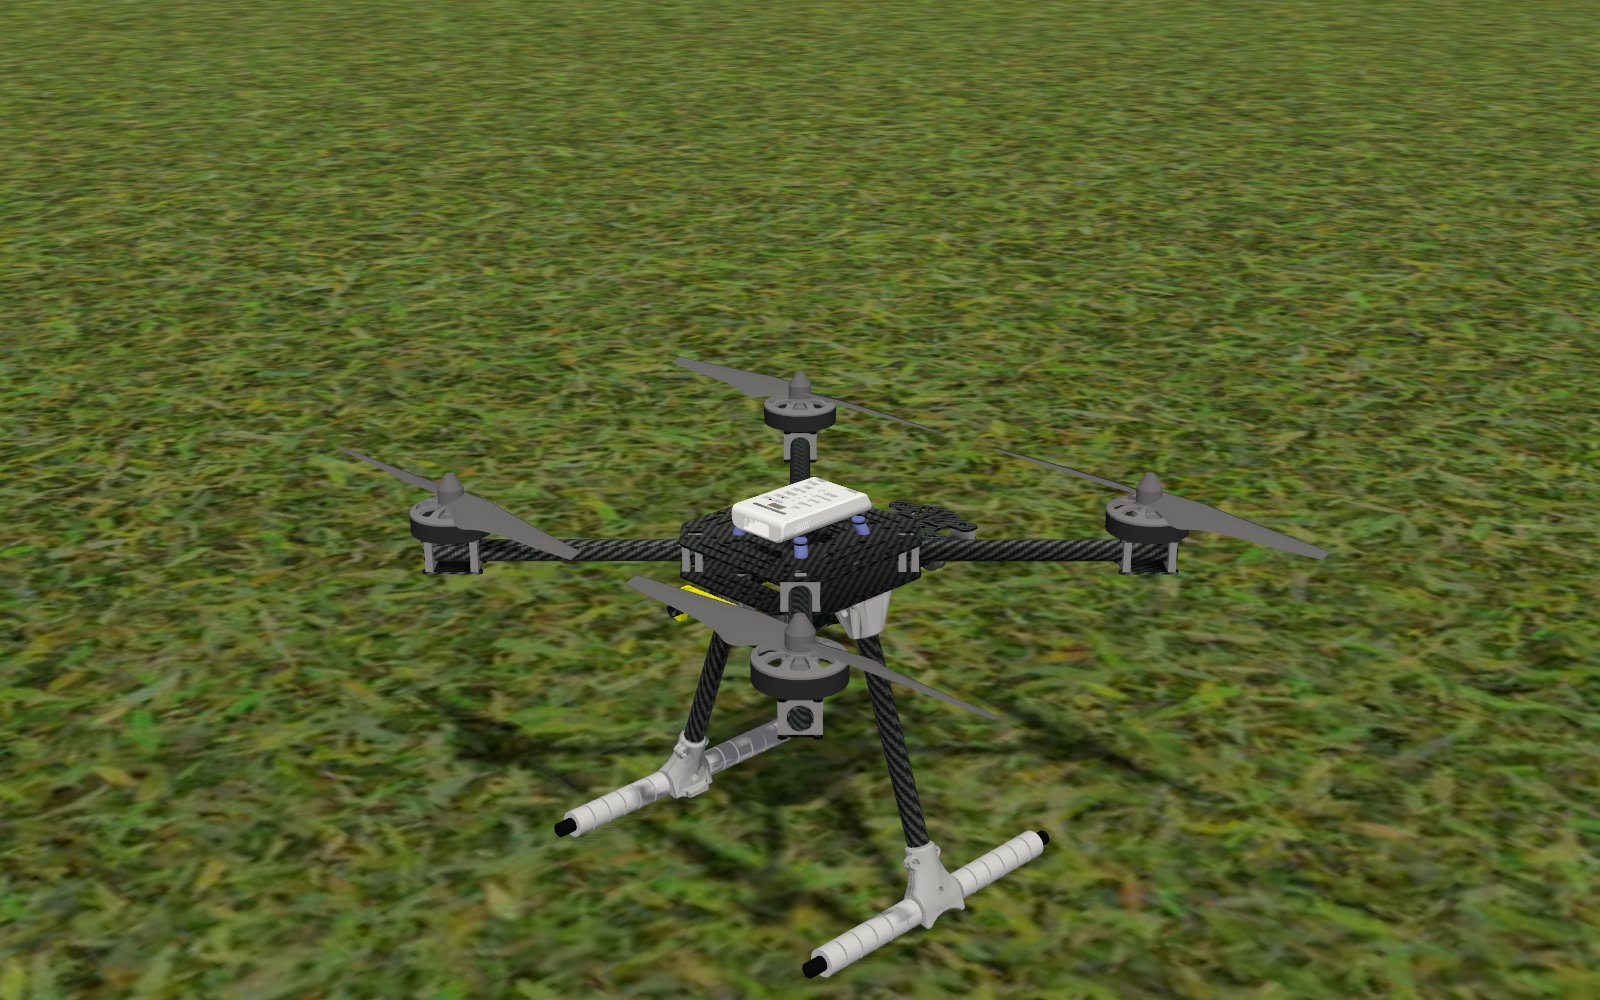
\includegraphics[height=0.78\textheight]{x500_tres_cuartos}};
    \begin{scope}[x={(img.south east)},y={(img.north west)},
        lb/.style={draw=azul,fill=white,rounded corners,font=\scriptsize,align=center,inner sep=2pt},
        fl/.style={-{Stealth},thick,azul}]
      \node[lb] (m) at (0.12,0.78) {\textbf{motor + hélice}\\4, uno por brazo};
      \draw[fl] (m) -- (0.28,0.50);
      \node[lb] (b) at (0.13,0.30) {\textbf{brazo}\\fibra de carbono};
      \draw[fl] (b) -- (0.36,0.44);
      \node[lb] (p) at (0.80,0.82) {\textbf{placa central}\\aquí va la Pixhawk (PX4)};
      \draw[fl] (p) -- (0.55,0.47);
      \node[lb] (t) at (0.85,0.22) {\textbf{tren de aterrizaje}};
      \draw[fl] (t) -- (0.60,0.12);
    \end{scope}
  \end{tikzpicture}\\
  \credito{El x500 de la simulación de PX4. Render propio de Gazebo}
\end{frame}

\begin{frame}{Cómo se mueve}
  \centering
  \begin{tikzpicture}[every node/.style={font=\scriptsize,align=center}]
    \foreach \x/\t/\d in {0/Subir/los 4 motores más rápido,3.6/Avanzar/se inclina hacia adelante:\\los de atrás más rápido,
        7.2/Ir a la derecha/se inclina a la derecha:\\los de la izquierda más rápido,10.8/Girar (yaw)/acelera un par diagonal\\y frena el otro} {
      \node at (\x,1.6) {\textbf{\t}};
      \node at (\x,0) {\dronarriba{2.1cm}};
      \node[text width=3.2cm] at (\x,-1.6) {\d};
    }
    % subir: 4 flechas hacia arriba (afuera de la página)
    \foreach \dx/\dy in {-0.55/0.55,0.55/0.55,-0.55/-0.55,0.55/-0.55} \fill[naranja] (\dx,\dy) circle (3.5pt);
    % avanzar: los de atrás
    \foreach \dx/\dy in {-0.55/-0.55,0.55/-0.55} \fill[naranja] (3.6+\dx,\dy) circle (3.5pt);
    \draw[-{Stealth},line width=2pt,verde] (3.6,0.4) -- (3.6,1.2);
    % derecha: los de la izquierda
    \foreach \dx/\dy in {-0.55/0.55,-0.55/-0.55} \fill[naranja] (7.2+\dx,\dy) circle (3.5pt);
    \draw[-{Stealth},line width=2pt,verde] (7.6,0) -- (8.5,0);
    % yaw: el par 1-2 (antihorario) más rápido -> el dron gira a la derecha
    \foreach \dx/\dy in {0.55/0.55,-0.55/-0.55} \fill[naranja] (10.8+\dx,\dy) circle (3.5pt);
    \draw[-{Stealth},line width=2pt,verde] (10.8,1.15) arc (90:20:1.15);
  \end{tikzpicture}
  \vspace{0.4em}

  \raggedright\small {\color{naranja}$\bullet$} = motor que acelera. El frente del dron es \textbf{arriba} en
  los dibujos. Nunca le dices a PX4 qué motor acelerar: le dices \textbf{a dónde ir} y él lo calcula.
\end{frame}

\begin{frame}{Los modos de vuelo: quién manda}
  \centering
  \begin{tikzpicture}[every node/.style={font=\scriptsize,align=center},
      md/.style={draw=azul,fill=azulclaro,rounded corners,text width=3.3cm,minimum height=1.45cm}]
    \node[md] at (0,1.0) {\textbf{Hold} \color{gris}(nav 4)\\\color{black}se queda quieto en el aire};
    \node[md,fill=yellow!25,draw=naranja] at (3.8,1.0) {\textbf{Offboard} \color{gris}(nav 14)\\\color{black}obedece a \textbf{tu nodo}};
    \node[md] at (7.6,1.0) {\textbf{Takeoff} \color{gris}(nav 17)\\\color{black}despega a una altura};
    \node[md] at (11.4,1.0) {\textbf{Land} \color{gris}(nav 18)\\\color{black}aterriza donde está};
    \node[md] at (0,-0.8) {\textbf{Return} \color{gris}(nav 5)\\\color{black}regresa a casa y aterriza};
    \node[md] at (3.8,-0.8) {\textbf{Position} \color{gris}(nav 2)\\\color{black}un piloto lo vuela\\con el control};
    \node[md] at (7.6,-0.8) {\textbf{Mission} \color{gris}(nav 3)\\\color{black}sigue waypoints\\hechos en QGC};
    \node[md] at (11.4,-0.8) {\textbf{Orbit} \color{gris}(nav 21)\\\color{black}da vueltas a un punto};
  \end{tikzpicture}
  \vspace{0.4em}

  \raggedright\small El modo actual sale en QGC y en \cmd{vehicle\_status\_v1.nav\_state}. Si tu nodo ``no hace
  nada'', lo primero es ver \textbf{en qué modo está}.
\end{frame}

\begin{frame}{Las reglas del piloto}
  \begin{columns}[c]
    \column{0.3\textwidth}\centering
    \dronlado{\linewidth}\\[0.4em]
    \small PX4 \textbf{siempre} está a cargo, aunque tu nodo esté mandando.
    \column{0.67\textwidth}\small
    \begin{enumerate}
      \item \textbf{No arma} si algo no está bien: sin GPS, con el estimador sin converger, sin
        QGroundControl conectado\ldots{} QGC dice la razón.
      \item \textbf{Armado} = motores girando. Si no despega en unos segundos, se \textbf{desarma solo}.
      \item En \textbf{Offboard}, si tu nodo deja de mandar mensajes \textasciitilde0.5 s, pasa a
        \textbf{Hold}.
      \item Con \textbf{batería baja} regresa a casa (Return) solo.
      \item Desde QGC \textbf{siempre} se le puede quitar el control a tu nodo: Hold, Land, Return.
    \end{enumerate}
  \end{columns}
\end{frame}
